\chapter{Probabilité}

\section{Rappels sur les calculs de probabilités}

\subsection{Expérience aléatoire}



\begin{definition}
	Une expérience est \textbf{aléatoire} lorsqu'elle a plusieurs résultats ou \textbf{issues} et que l'on ne peut pas prévoir quel résultat se produira.

	L'ensemble de toutes les \textbf{issues} d'une expérience s'appelle \textbf{l'univers} noté $\Omega$ (ou parfois $U$).
	\begin{center}
		\begin{tikzpicture}[
				% Définition des styles
				box/.style={rectangle, draw=blue!60, fill=blue!5, thick, rounded corners, minimum height=3.7cm, minimum width=10cm, align=center},
				issue/.style={circle, draw=orange!80, fill=orange!20, thick, inner sep=4pt, font=\small\bfseries},
				exp/.style={ellipse, draw=purple!80, fill=purple!10, thick, minimum height=1.2cm, minimum width=2.8cm, align=center, font=\small}
			]

			% 1. L'Expérience Aléatoire (à gauche)
			\node[exp] (experience) at (-6.5, 0) {\textbf{Expérience}\\\textbf{Aléatoire}\\ \textit{(Résultat imprévisible)}};

			% 2. L'Univers Oméga (la grande boîte à droite)
			\node[box] (univers) at (2.5, 0) {};
			% Étiquette de l'Univers
			\node[anchor=north west, blue!80!black, font=\bfseries] at (univers.north west) {\,$\Omega$ (L'Univers)};
			\node[anchor=south, blue!80!black, font=\small\itshape] at (univers.south) {Ensemble de tous les résultats possibles};

			% 3. Les Issues (à l'intérieur de l'univers)
			\node[issue] (i1) at (0.2, 0.6)  {Issue 1};
			\node[issue] (i2) at (3.8, 0.5)  {Issue 2};
			\node[issue] (i3) at (2.2, -0.6) {Issue 3};
			\node[issue, dashed, draw=orange!50, fill=orange!5, text=orange!60] (i4) at (6.3, -0.6) {Issue $n$};

			% Petits points de suspension entre les issues
			\path (i3) -- (i4) node [midway, font=\bfseries, text=orange!70] {\dots};

			% 4. Flèches de l'expérience vers les issues (Processus aléatoire)
			\draw[-{Stealth[scale=1.2]}, thick, purple!70, dashed] (experience.east) -- (i1.west);
			\draw[-{Stealth[scale=1.2]}, thick, purple!70, dashed] (experience.east) -- (i2.west) ; %node[midway, above, sloped, text=purple!90, font=\scriptsize\bfseries] {?};
			\draw[-{Stealth[scale=1.2]}, thick, purple!70, dashed] (experience.east) -- (i3.west);
			\draw[-{Stealth[scale=1.2]}, thick, purple!70, dashed] (experience.east) -- (i4.west);

		\end{tikzpicture}
	\end{center}
\end{definition}

\begin{ex}
	\leavevmode\vspace{-\baselineskip}
	\begin{itemize}
		\item On lance une pièce de monnaie et on regarde la face supérieure.
		\item On lance un dé à six faces et on regarde le nombre de points inscrits sur la face du dessus.
		\item On fait tourner une roue marquée sur ses secteurs de couleurs différentes et on regarde la couleur du secteur marqué par la flèche.
	\end{itemize}
\end{ex}

\subsection{Évènement}

\begin{definition}
	Un \textbf{évènement} est constitué d'une ou plusieurs issues d'une même expérience aléatoire.
\end{definition}

\begin{exemple}
	On lance un dé à six faces.
	\begin{itemize}
		\item \og{}Obtenir un chiffre pair\fg{} est l'évènement constitué des issues : 2 ; 4 et 6.
		\item \og{}Obtenir un chiffre inférieur ou égal à 2\fg{} est l'évènement constitué des issues : 1 et 2.
	\end{itemize}
\end{exemple}

\subsection{Probabilité}

\begin{definition}
	La \textbf{probabilité} d'un évènement est un nombre compris entre $0$ et $1$ qui exprime \og{}la chance\fg{} qu'a un évènement de se produire.
\end{definition}

\begin{exemple}
	Dire que la probabilité d'un évènement est de $0,8$ signifie que cet évènement a $8$ chances sur $10$ ou $80$\% de chance de se produire.
\end{exemple}
\newpage

\begin{remarque}
	Soit un événement $E$ définit sur un univers $\Omega$.
	\begin{itemize}
		\item Un évènement dont la probabilité est égale à $0$ est un évènement \textbf{impossible}.
		\item Un évènement dont la probabilité est égale à $1$ est un évènement \textbf{certain}.
		\item Lorsque chaque issue a autant de chance de se produire, on dit qu'il y a \textbf{équiprobabilité}.
	\end{itemize}
\end{remarque}

\begin{propriete}
	En cas d'équiprobabilité, la probabilité d'un évènement $A$ est :
	\[
		P(A) = \frac{\text{Nombre d'issues favorables à } A}{\text{Nombre d'issues total}}
	\]
\end{propriete}

\begin{methode}[Calculer une probabilité (1)]
	On lance un dé à 6 faces. On considère les évènements :
	\begin{itemize}
		\item $E$ = \og{}On obtient un 3\fg{}
		\item $F$ = \og{}On obtient un chiffre pair\fg{}
		\item $G$ = \og{}On obtient un chiffre strictly supérieur à 3\fg{}
	\end{itemize}
	Calculer la probabilité de ces évènements.
\end{methode}

\begin{proof}[Correction]
	~
	\begin{itemize}
		\item Nombre d'issues favorables à $E$ : 1. Nombre d'issues total : 6. En effet, le dé a 6 faces.
		      \[ P(E) = \frac{1}{6} \]
		\item Nombre d'issues favorables à $F$ : 3 (2, 4 ou 6).
		      \[ P(F) = \frac{3}{6} = \frac{1}{2} \]
		\item Nombre d'issues favorables à $G$ : 3 (4, 5 ou 6).
		      \[ P(G) = \frac{3}{6} = \frac{1}{2} \]
	\end{itemize}
\end{proof}

\begin{methode}[Calculer une probabilité (2)]
	On tire une carte dans un jeu de 32 cartes. Soit $E$ l'évènement : \og{}On tire un as\fg{}. \\
	Quelle est la probabilité de l'événement $E$ ?
\end{methode}

\begin{proof}[Correction]
	Il y a 32 issues possibles car il existe 32 façons différentes de tirer une carte. \\
	L'évènement $E$ possède 4 issues possibles : As de cœur, as de carreau, as de trèfle, as de pique. \\
	La probabilité de l'événement $E$ est donc égale à : $P(E) = \frac{4}{32} = \frac{1}{8}$.
\end{proof}

\section{Évènement contraire, réunion, intersection}

\subsection{Évènement contraire}

\begin{definition}
	L'événement contraire de $A$, noté $\overline{A}$, est l'ensemble de toutes les issues n'appartenant pas à $A$.
\end{definition}

\begin{exemple}
	\leavevmode \vspace{-\baselineskip}
	\begin{itemize}
		\item L'évènement contraire de l'évènement \og{}Obtenir un chiffre pair\fg{} est l'événement \og{}Obtenir un chiffre impair\fg{}.
		\item L'évènement contraire de l'évènement \og{}Obtenir un chiffre inférieur ou égal à 2\fg{} est l'événement constitué des issues 3 ; 4 ; 5 et 6.
	\end{itemize}
\end{exemple}

\begin{propriete}
	La probabilité de l'événement contraire d'un événement $A$ est :
	\[
		P(\overline{A}) = 1 - P(A)
	\]
\end{propriete}

\begin{exemple}
	La probabilité de gagner au tennis contre Evelyne est : $P(G) = 0,2$. \\
	Alors la probabilité de perdre (évènement contraire) est :
	\[
		P(\overline{G}) = 1 - P(G) = 1 - 0,2 = 0,8.
	\]
\end{exemple}

\subsection{Loi de probabilité}

\begin{exemple}
	Une urne contient 6 boules vertes, 3 boules jaunes et 11 boules noires. \\
	On tire une boule au hasard et on note sa couleur. \\
	Le tableau suivant présente les probabilités de toutes les issues de l'expérience, on l'appelle \textbf{loi de probabilité}.

	\begin{center}
		\begin{tabular}{|c|c|c|c|}
			\hline
			\textbf{Issues}       & Boule verte          & Boule jaune           & Boule noire            \\
			\hline
			\textbf{Probabilités} & $\frac{6}{20} = 0,3$ & $\frac{3}{20} = 0,15$ & $\frac{11}{20} = 0,55$ \\
			\hline
		\end{tabular}
	\end{center}
\end{exemple}

\begin{propriete}
	La somme des probabilités de toutes les issues est égale à 1.
\end{propriete}

\begin{exemple}
	$P(\text{Boule verte}) + P(\text{Boule jaune}) + P(\text{Boule noire}) = 0,3 + 0,15 + 0,55 = 1$.
\end{exemple}

\begin{methode}[Utiliser une loi de probabilité]
	On tire au hasard un jeton dans le sac contenant des jetons numérotés de 1 à 5. \\
	Le tableau présente les probabilités de toutes les issues (loi de probabilité).

	\begin{center}
		\begin{tabular}{|c|c|c|c|c|c|}
			\hline
			\textbf{Issues}       & 1              & 2              & 3 & 4              & 5              \\
			\hline
			\textbf{Probabilités} & $\frac{1}{15}$ & $\frac{4}{15}$ & ? & $\frac{3}{15}$ & $\frac{4}{15}$ \\
			\hline
		\end{tabular}
	\end{center}

	\begin{enumerate}[label=\alph*)]
		\item Compléter le tableau de la loi de probabilité.
		\item Calculer la probabilité de l'évènement $E$ : \og{}Tirer un chiffre pair\fg{}.
		\item Décrire l'évènement $\overline{E}$ puis calculer sa probabilité.
	\end{enumerate}

	\begin{correction}
		\leavevmode\vspace{-\baselineskip}
		\begin{enumerate}[label=\alph*)]
			\item La somme des probabilités de toutes les issues est égale à 1, donc :
			      \[
				      P(1) + P(2) + P(3) + P(4) + P(5) = 1
			      \]
			      \[
				      \frac{1}{15} + \frac{4}{15} + P(3) + \frac{3}{15} + \frac{4}{15} = 1 \implies P(3) + \frac{12}{15} = 1
			      \]
			      \[
				      P(3) = 1 - \frac{12}{15} = \frac{15}{15} - \frac{12}{15} = \frac{3}{15} = \frac{1}{5}
			      \]
			\item L'évènement $E$ possède deux issues : 2 et 4. \\
			      Donc, d'après le tableau : $P(E) = \frac{4}{15} + \frac{3}{15} = \frac{7}{15}$.
			\item $\overline{E}$ est l'évènement : \og{}Ne pas tirer un chiffre pair\fg{}.
			      \[
				      P(\overline{E}) = 1 - P(E) = 1 - \frac{7}{15} = \frac{8}{15}.
			      \]
		\end{enumerate}
	\end{correction}
\end{methode}

\subsection{Réunion et intersection de deux événements}

\begin{exemple}
	Soit les évènements : $A = \{1 ; 2\}$ et $B = \{1 ; 3 ; 4\}$. \\
	Alors $A \cap B = \{1\}$ et $A \cup B = \{1 ; 2 ; 3 ; 4\}$.
\end{exemple}

\begin{methode}[Calculer la probabilité d'une intersection]
	On lance un dé à six faces et on considère les événements suivants :
	\begin{itemize}
		\item $A$ : \og{}Obtenir un multiple de 2\fg{}.
		\item $B$ : \og{}Obtenir un nombre inférieur ou égal à 4\fg{}.
	\end{itemize}
	\begin{enumerate}[label=\alph*)]
		\item Décrire par une phrase l'évènement $A \cap B$.
		\item Déterminer les issues des évènements : $A$, $B$ et $A \cap B$.
		\item Calculer $P(A)$, $P(B)$, $P(A \cap B)$.
	\end{enumerate}
\end{methode}

\begin{correction}
	\leavevmode\vspace{-\baselineskip}
	\begin{enumerate}[label=\alph*)]
		\item $A \cap B$ : \og{}Obtenir un multiple de 2 inférieur ou égal à 4.\fg{}
		\item On a : $A = \{2 ; 4 ; 6\}$ et $B = \{1 ; 2 ; 3 ; 4\}$. Donc $A \cap B = \{2 ; 4\}$.
		\item $P(A) = \frac{3}{6} = \frac{1}{2}$, $P(B) = \frac{4}{6} = \frac{2}{3}$, $P(A \cap B) = \frac{2}{6} = \frac{1}{3}$.
	\end{enumerate}
\end{correction}

\begin{theoreme}
	\[
		P(A \cup B) = P(A) + P(B) - P(A \cap B)
	\]
\end{theoreme}

\begin{methode}[Calculer la probabilité d'une réunion]
	On lance un dé à six faces et on considère les événements suivants : \\
	$A$ : \og{}On obtient un nombre impair\fg{} \\
	$B$ : \og{}On obtient un multiple de 3\fg{}
	\begin{enumerate}[label=\alph*)]
		\item Calculer $P(A)$, $P(B)$, $P(A \cap B)$.
		\item Calculer la probabilité de l'événement $A \cup B$. Interpréter le résultat.
	\end{enumerate}
\end{methode}

\begin{proof}[Correction]
	\begin{enumerate}[label=\alph*)]
		\item On a $A = \{1 ; 3 ; 5\}$ et $B = \{3 ; 6\}$, donc $P(A) = \frac{3}{6} = \frac{1}{2}$ et $P(B) = \frac{2}{6} = \frac{1}{3}$. \\
		      On a $A \cap B = \{3\}$, donc $P(A \cap B) = \frac{1}{6}$.
		\item $P(A \cup B) = P(A) + P(B) - P(A \cap B) = \frac{1}{2} + \frac{1}{3} - \frac{1}{6} = \frac{3}{6} + \frac{2}{6} - \frac{1}{6} = \frac{4}{6} = \frac{2}{3}$. \\
		      La probabilité d'obtenir un nombre impair ou un multiple de 3 est égale à $\frac{2}{3}$.
	\end{enumerate}
\end{proof}

\section{Arbre pondéré}

\begin{exemple}
	Dans un sac, on dépose quatre jetons : un bleu, un rouge, un jaune et un vert. \\
	En tirant au hasard un jeton du sac, on a quatre issues possibles. On représente les issues sur un schéma appelé \textbf{arbre pondéré} ou \textbf{arbre de probabilité}.

	\begin{center}
		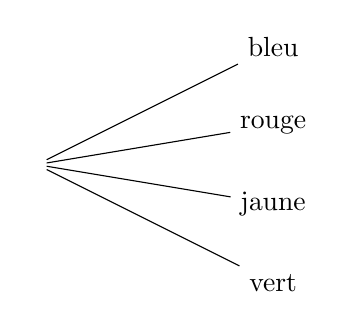
\begin{tikzpicture}[grow=right, sloped, level distance=3cm, sibling distance=1cm]
			\node {}
			child { node {vert} }
			child { node {jaune} }
			child { node {rouge} }
			child { node {bleu} };
		\end{tikzpicture}
	\end{center}
\end{exemple}

\begin{methode}[Utiliser un arbre pondéré]
	On lance deux fois de suite une pièce de monnaie. Il s'agit d'une expérience aléatoire à deux épreuves. \\
	Soit $E$ l'événement : \og{}On obtient au moins une fois PILE.\fg{} \\
	Calculer $P(E)$ en utilisant un arbre pondéré.
\end{methode}

\begin{proof}[Correction]
	On construit un arbre présentant les résultats possibles aux deux épreuves de l'expérience (P pour PILE et F pour FACE).

	\begin{center}
		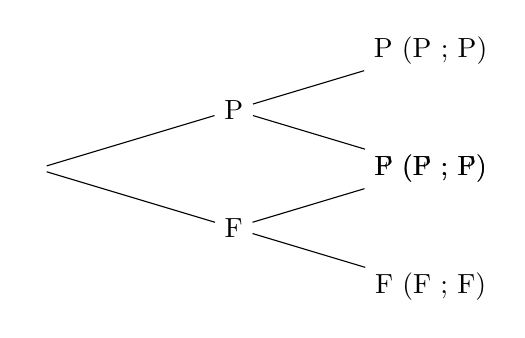
\begin{tikzpicture}[grow=right, sloped, level distance=2.5cm, sibling distance=1.5cm]
			\node {}
			child {
					node {F}
					child { node {F (F ; F)} }
					child { node {P (F ; P)} }
				}
			child {
					node {P}
					child { node {F (P ; F)} }
					child { node {P (P ; P)} }
				};
		\end{tikzpicture}
	\end{center}

	\begin{itemize}
		\item On compte 4 issues en tout : (P ; P), (P ; F), (F ; P) et (F ; F).
		\item L'événement $E$ possède 3 issues : (P ; P), (P ; F) et (F ; P).
	\end{itemize}
	La probabilité de $E$ est donc égale à $\frac{3}{4}$.
\end{proof}

\section{Probabilités conditionnelles}

\subsection{Calcul à l'aide d'un tableau croisé}

\begin{definition}
	On appelle \textbf{probabilité conditionnelle de $B$ sachant $A$}, la probabilité que l'événement $B$ se réalise sachant que l'événement $A$ est réalisé. On la note : $P_A(B)$.
\end{definition}

\begin{propriete}
	\[
		P_A(B) = \frac{\text{Card}(A \cap B)}{\text{Card}(A)}
	\]
\end{propriete}

\begin{methode}[Calculer une probabilité conditionnelle à l'aide d'un tableau]
	Un laboratoire pharmaceutique a réalisé des tests sur 800 patients atteints d'une maladie. Certains sont traités avec le médicament A, d'autres avec le médicament B.

	\begin{center}
		\begin{tabular}{|c|c|c|c|}
			\hline
			          & Médicament A & Médicament B & Total \\
			\hline
			Guéri     & 383          & 291          & 674   \\
			\hline
			Non guéri & 72           & 54           & 126   \\
			\hline
			Total     & 455          & 345          & 800   \\
			\hline
		\end{tabular}
	\end{center}

	\begin{enumerate}
		\item On choisit au hasard un patient : $A$ : \og{}Médicament A\fg{}, $G$ : \og{}Guéri\fg{}. \\
		      Calculer : a) $P(A)$ \quad b) $P(G)$ \quad c) $P(G \cap A)$ \quad d) $P(\overline{G} \cap A)$.
		\item a) Calculer la probabilité que le patient ait pris le médicament A sachant qu'il est guéri. \\
		      b) Calculer la probabilité que le patient soit guéri sachant qu'il a pris le médicament B.
	\end{enumerate}
\end{methode}

\begin{proof}[Correction]
	\begin{enumerate}
		\item
		      a) $P(A) = \frac{455}{800} \approx 0,57 = 57\%$ \\
		      b) $P(G) = \frac{674}{800} \approx 0,84 = 84\%$ \\
		      c) $P(G \cap A) = \frac{383}{800} \approx 0,48 = 48\%$ \\
		      d) $P(\overline{G} \cap A) = \frac{72}{800} \approx 0,09 = 9\%$
		\item
		      a) $P_G(A) = \frac{383}{674} \approx 0,57 = 57\%$. \\
		      b) $P_B(G) = \frac{291}{345} \approx 0,84 = 84\%$.
	\end{enumerate}
\end{proof}

\subsection{Calcul à l'aide de la formule}

\begin{propriete}
	\[
		P_A(B) = \frac{P(A \cap B)}{P(A)}
	\]
\end{propriete}

\begin{methode}[Calculer une probabilité conditionnelle à l'aide de la formule]

	On tire une carte au hasard dans un jeu de 32 cartes. \\
	$A$ : \og{}Le résultat est un cœur\fg{} ; $B$ : \og{}Le résultat est un valet\fg{}. \\
	Calculer $P_A(B)$.
\end{methode}

\begin{proof}[Correction]
	$P(A) = \frac{8}{32} = 0,25$ et $P(A \cap B) = \frac{1}{32} = 0,03125$. \\
	Donc $P_A(B) = \frac{P(A \cap B)}{P(A)} = \frac{0,03125}{0,25} = 0,125$.
\end{proof}

\subsection{Calcul à l'aide d'un arbre}

\begin{propriete}
	Soit $A$ et $B$ deux événements avec $P(A) \neq 0$.
	\begin{itemize}
		\item $P_A(\overline{B}) = 1 - P_A(B)$
		\item $P(A \cap B) = P(A) \times P_A(B)$
	\end{itemize}
\end{propriete}

\begin{methode}[Construire un arbre pondéré]
\end{methode}

\section{Loi des grands nombres}

\begin{definition}
	Un \textbf{échantillon} de taille $n$ est constitué des résultats de $n$ répétitions indépendantes de la même expérience.
\end{definition}

\begin{methode}[Estimer une probabilité à l'aide de la loi des grands nombres]

	Voici un programme Python permettant de mesurer la probabilité d'obetnir \epsdice{1} ou \epsdice{6}

	\begin{lstlisting}
from random import *

def de(n):
    s = 0
    for k in range(n):
        r = randint(1, 6)
        if r == 1 or r == 6:
            s = s + 1
    return(s / n)
\end{lstlisting}
\end{methode}

\begin{propriete}[Loi des grands nombres]
	Lorsque $n$ devient grand, la fréquence observée est le plus souvent proche de la probabilité théorique.
\end{propriete}
